% !TEX TS-program = pdflatexmk
\documentclass[12pt]{article}

% Layout.
\usepackage[top=.75in, bottom=0.75in, left=.75in, right=.75in, headheight=1in, headsep=6pt]{geometry}

% Fonts.
\usepackage{mathptmx}
\usepackage[scaled=0.86]{helvet}
\renewcommand{\emph}[1]{\textsf{\textbf{#1}}}

% Misc packages.
\usepackage{amsmath,amssymb,latexsym}
\usepackage{graphicx,tikz}
\usepackage{array}
\usepackage{xcolor}
\usepackage{multicol}
\usepackage{tabularx,colortbl}
\usepackage{enumitem}
%to make tikz pics work
\usepackage{tikz,pgfplots}
\usetikzlibrary{arrows}
\newcommand{\midarrow}{\tikz \draw[-triangle 90] (0,0) -- +(.1,0);}

\usepackage[colorlinks=true]{hyperref}

% Paragraph spacing
\parindent 0pt
\parskip 6pt plus 1pt
\def\tableindent{\hskip 0.5 in}
\def\ts{\hskip 1.5 em}

\usepackage{fancyhdr}
\pagestyle{fancy} 
\lhead{\large\sf\textbf{MATH 663 }}
\rhead{\large\sf\textbf{Fall 2023}}
\chead{\large\sf\textbf{Midterm 2}}

\newcommand{\localhead}[1]{\par\smallskip\textbf{#1}\nobreak\\}%
\def\heading#1{\localhead{\large\emph{#1}}}
\def\subheading#1{\localhead{\emph{#1}}}

%% Special Math Symbol shortcuts
\newcommand{\bbN}{\mathbb{N}}
\newcommand{\rad}{\text{rad}}
\newcommand{\diam}{\text{diam}}

%\newenvironment{clist}%
%{\bgroup\parskip 0pt\begin{list}{$\bullet$}{\partopsep 4pt\topsep 0pt\itemsep -2pt}}%
%{\end{list}\egroup}%

\usetikzlibrary{calc,arrows.meta}
\usetikzlibrary{arrows}
\newcommand{\marrow}{\tikz \draw[-triangle 90] (0,0) -- +(.1,0);}


\begin{document}

\textbf{Directions:} 
\begin{itemize}
	\item You have 2 hours to complete all 6 of the problems below. 
	\item Books, notes or other aids are not allowed. 
	\item To receive full credit, proofs must be formal.
	\item Paper will be provided for you. Please put your answer to each problems on a separate sheet of paper.
\end{itemize}

\hrulefill

\begin{enumerate}

\item Let $G$ be a simple graph such that  $\chi(G)=k.$ Let $c: V(G) \to [k]$ be a $k$-coloring of the vertex set of $G.$ Prove that for every $i \in [k],$ there exists at least one vertex assigned color $i$ that is adjacent to at least one vertex of each of the other $k-1$ colors.

\item Prove that if $G$ is $r$-regular and $\kappa(G)=1,$ then $\chi'(G) > r.$ (Recall that $\kappa(G)$ is the connectivity of a graph.)

\item 
	\begin{enumerate}
	\item Describe the graph, $T^r(n)$, the Tur\'{a}n graph, as described in our text.
	\item State Tur\'{a}n's Theorem.
	\item Suppose that $n\geq 2r.$ Show that $|E(T^r(n))|={ r \choose 2}+(n-r)(r-1) +|E(T^r(n-r))|.$
	\end{enumerate}
\item Suppose that $G$ is planar and triangle-free. Prove that $G$ has a vertex of degree at most 3.

\item Suppose that $G$ is a graph such that every subgraph of $G$ contains a vertex of degree $k$ or less. Prove that the chromatic number of $G$ is at most $k+1.$

\vfill

See the 6th problem on networks on the next page!

\vfill

\newpage
\item In the network below, the capacity and flow value for each edge are represented with an ordered pair: $(\text{capacity},\text{flow}).$ Assume the capacity of every edge is the same regardless of direction. (So $c(sa)=c(as)=3.$) Assume the arrows indicate the direction of positive flow. (So, $f(sa)=3$ and $f(as)=-3.$)

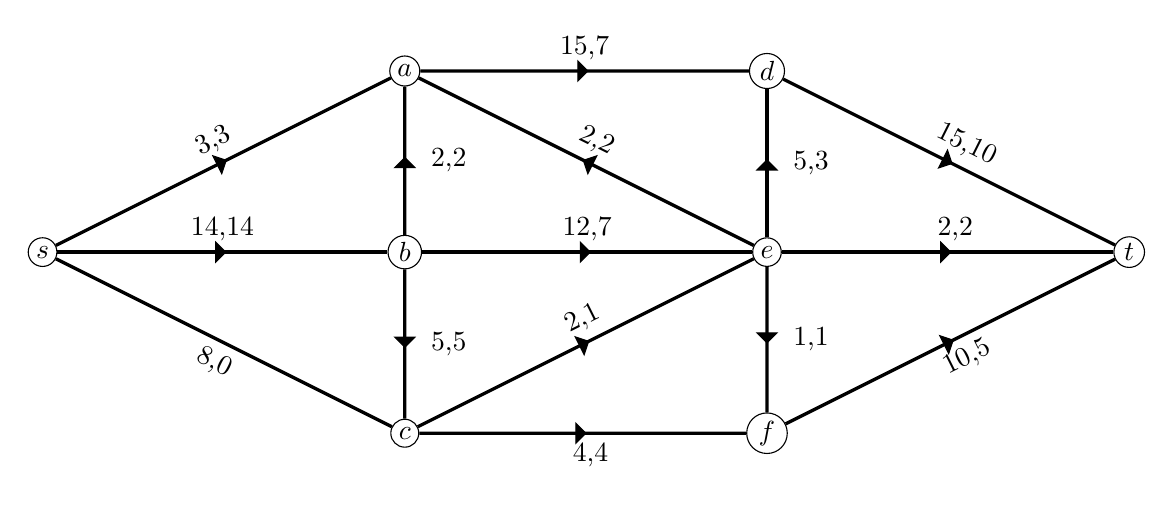
\begin{tikzpicture}[scale=2.3,every node/.style={draw,circle, inner sep=.05 cm}]
	
	\node (s) at (0,0){$s$};
	\node (a) at (2,1){$a$};
	\node (b) at (2,0){$b$};
	\node (c) at (2,-1){$c$};
	\node (d) at (4,1){$d$};
	\node (e) at (4,0){$e$};
	\node (f) at (4,-1){$f$};
	\node (t) at (6,0){$t$};
	\begin{scope}[very thick, every node/.style={sloped,allow upside down}]
	%edges
	\draw (s) -- node{\marrow} node[above]{3,3} (a);
	\draw (s) -- node{\marrow} node[above]{14,14} (b);
	\draw (s) -- node[below]{8,0} (c);
	\draw (a) -- node{\marrow} node[above]{15,7} (d);
	\draw (e) -- node{\marrow}node[above,rotate=180]{2,2} (a);
	\draw (b) -- node{\marrow}node[right,rotate=-90]{\: 2,2 \quad} (a);
	\draw (b) -- node{\marrow}node[above]{12,7} (e);
	\draw (b) -- node{\marrow}node[right,rotate=90]{\: 5,5} (c);
	\draw (c) -- node{\marrow}node[above]{\: 2,1} (e);
	\draw (c) -- node{\marrow}node[below]{\: 4,4} (f);
	\draw (e) -- node{\marrow}node[right,rotate=-90]{\: 5,3} (d);
	\draw (d) -- node{\marrow}node[above]{\: 15,10} (t);
	\draw (e) -- node{\marrow}node[right,rotate=90]{\: 1,1} (f);
	\draw (e) -- node{\marrow}node[above]{\: 2,2} (t);
	\draw (f) -- node{\marrow}node[below]{\: 10,5} (t);
	
	\end{scope}
	\end{tikzpicture}

Use the iterative process from the Ford-Fulkerson Theorem to augment the existing flow until a maximum flow is obtained. You can illustrate your iterative process using the figure(s) below. Demonstrate that your flow has maximum value by finding an appropriate vertex cut $S.$\\

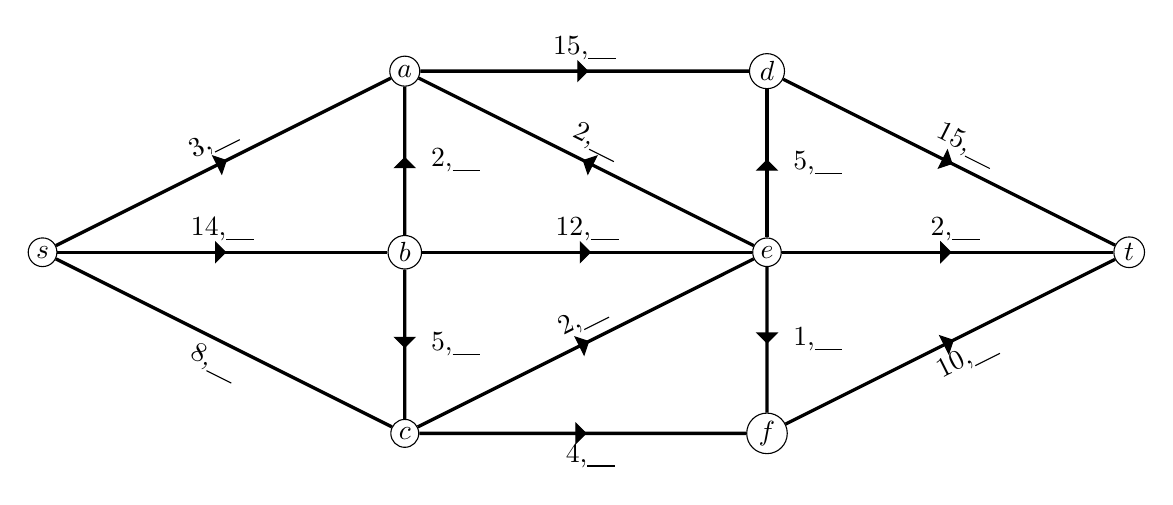
\begin{tikzpicture}[scale=2.3,every node/.style={draw,circle, inner sep=.05 cm}]
	
	\node (s) at (0,0){$s$};
	\node (a) at (2,1){$a$};
	\node (b) at (2,0){$b$};
	\node (c) at (2,-1){$c$};
	\node (d) at (4,1){$d$};
	\node (e) at (4,0){$e$};
	\node (f) at (4,-1){$f$};
	\node (t) at (6,0){$t$};
	\begin{scope}[very thick, every node/.style={sloped,allow upside down}]
	%edges
	\draw (s) -- node{\marrow} node[above]{3,\underline{\quad}} (a);
	\draw (s) -- node{\marrow} node[above]{14,\underline{\quad}} (b);
	\draw (s) -- node[below]{8,\underline{\quad}} (c);
	\draw (a) -- node{\marrow} node[above]{15,\underline{\quad}} (d);
	\draw (e) -- node{\marrow}node[above,rotate=180]{2,\underline{\quad}} (a);
	\draw (b) -- node{\marrow}node[right,rotate=-90]{\: 2,\underline{\quad} \quad} (a);
	\draw (b) -- node{\marrow}node[above]{12,\underline{\quad}} (e);
	\draw (b) -- node{\marrow}node[right,rotate=90]{\: 5,\underline{\quad}} (c);
	\draw (c) -- node{\marrow}node[above]{\: 2,\underline{\quad}} (e);
	\draw (c) -- node{\marrow}node[below]{\: 4,\underline{\quad}} (f);
	\draw (e) -- node{\marrow}node[right,rotate=-90]{\: 5,\underline{\quad}} (d);
	\draw (d) -- node{\marrow}node[above]{\: 15,\underline{\quad}} (t);
	\draw (e) -- node{\marrow}node[right,rotate=90]{\: 1,\underline{\quad}} (f);
	\draw (e) -- node{\marrow}node[above]{\: 2,\underline{\quad}} (t);
	\draw (f) -- node{\marrow}node[below]{\: 10,\underline{\quad}} (t);
	
	\end{scope}
	\end{tikzpicture}


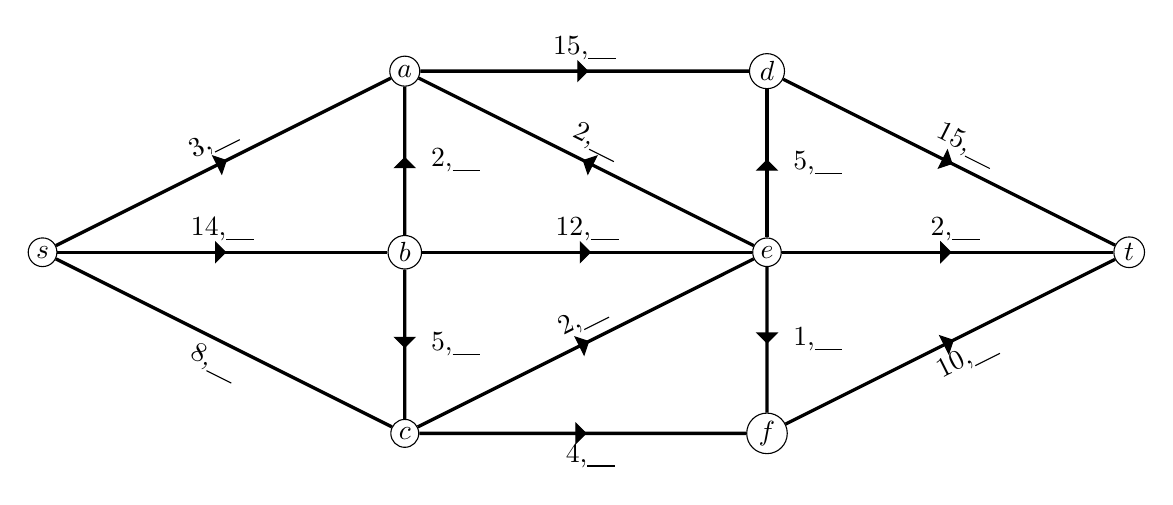
\begin{tikzpicture}[scale=2.3,every node/.style={draw,circle, inner sep=.05 cm}]
	
	\node (s) at (0,0){$s$};
	\node (a) at (2,1){$a$};
	\node (b) at (2,0){$b$};
	\node (c) at (2,-1){$c$};
	\node (d) at (4,1){$d$};
	\node (e) at (4,0){$e$};
	\node (f) at (4,-1){$f$};
	\node (t) at (6,0){$t$};
	\begin{scope}[very thick, every node/.style={sloped,allow upside down}]
	%edges
	\draw (s) -- node{\marrow} node[above]{3,\underline{\quad}} (a);
	\draw (s) -- node{\marrow} node[above]{14,\underline{\quad}} (b);
	\draw (s) -- node[below]{8,\underline{\quad}} (c);
	\draw (a) -- node{\marrow} node[above]{15,\underline{\quad}} (d);
	\draw (e) -- node{\marrow}node[above,rotate=180]{2,\underline{\quad}} (a);
	\draw (b) -- node{\marrow}node[right,rotate=-90]{\: 2,\underline{\quad} \quad} (a);
	\draw (b) -- node{\marrow}node[above]{12,\underline{\quad}} (e);
	\draw (b) -- node{\marrow}node[right,rotate=90]{\: 5,\underline{\quad}} (c);
	\draw (c) -- node{\marrow}node[above]{\: 2,\underline{\quad}} (e);
	\draw (c) -- node{\marrow}node[below]{\: 4,\underline{\quad}} (f);
	\draw (e) -- node{\marrow}node[right,rotate=-90]{\: 5,\underline{\quad}} (d);
	\draw (d) -- node{\marrow}node[above]{\: 15,\underline{\quad}} (t);
	\draw (e) -- node{\marrow}node[right,rotate=90]{\: 1,\underline{\quad}} (f);
	\draw (e) -- node{\marrow}node[above]{\: 2,\underline{\quad}} (t);
	\draw (f) -- node{\marrow}node[below]{\: 10,\underline{\quad}} (t);
	
	\end{scope}
	\end{tikzpicture}

	

\end{enumerate}

\end{document}